\section{Methods} \label{sec:usbe_lung_methods}%
In this section, we describe the set of numerical experiments
performed to investigate the fundamental fluid dynamics associated
with acoustically-accelerated, perturbed liquid-gas interfaces and
\ac{US}-induced \ac{LH}.

\subsection{Problem set-up}
\label{subsec:setup}
\begin{figure}[t]
  \centering
%  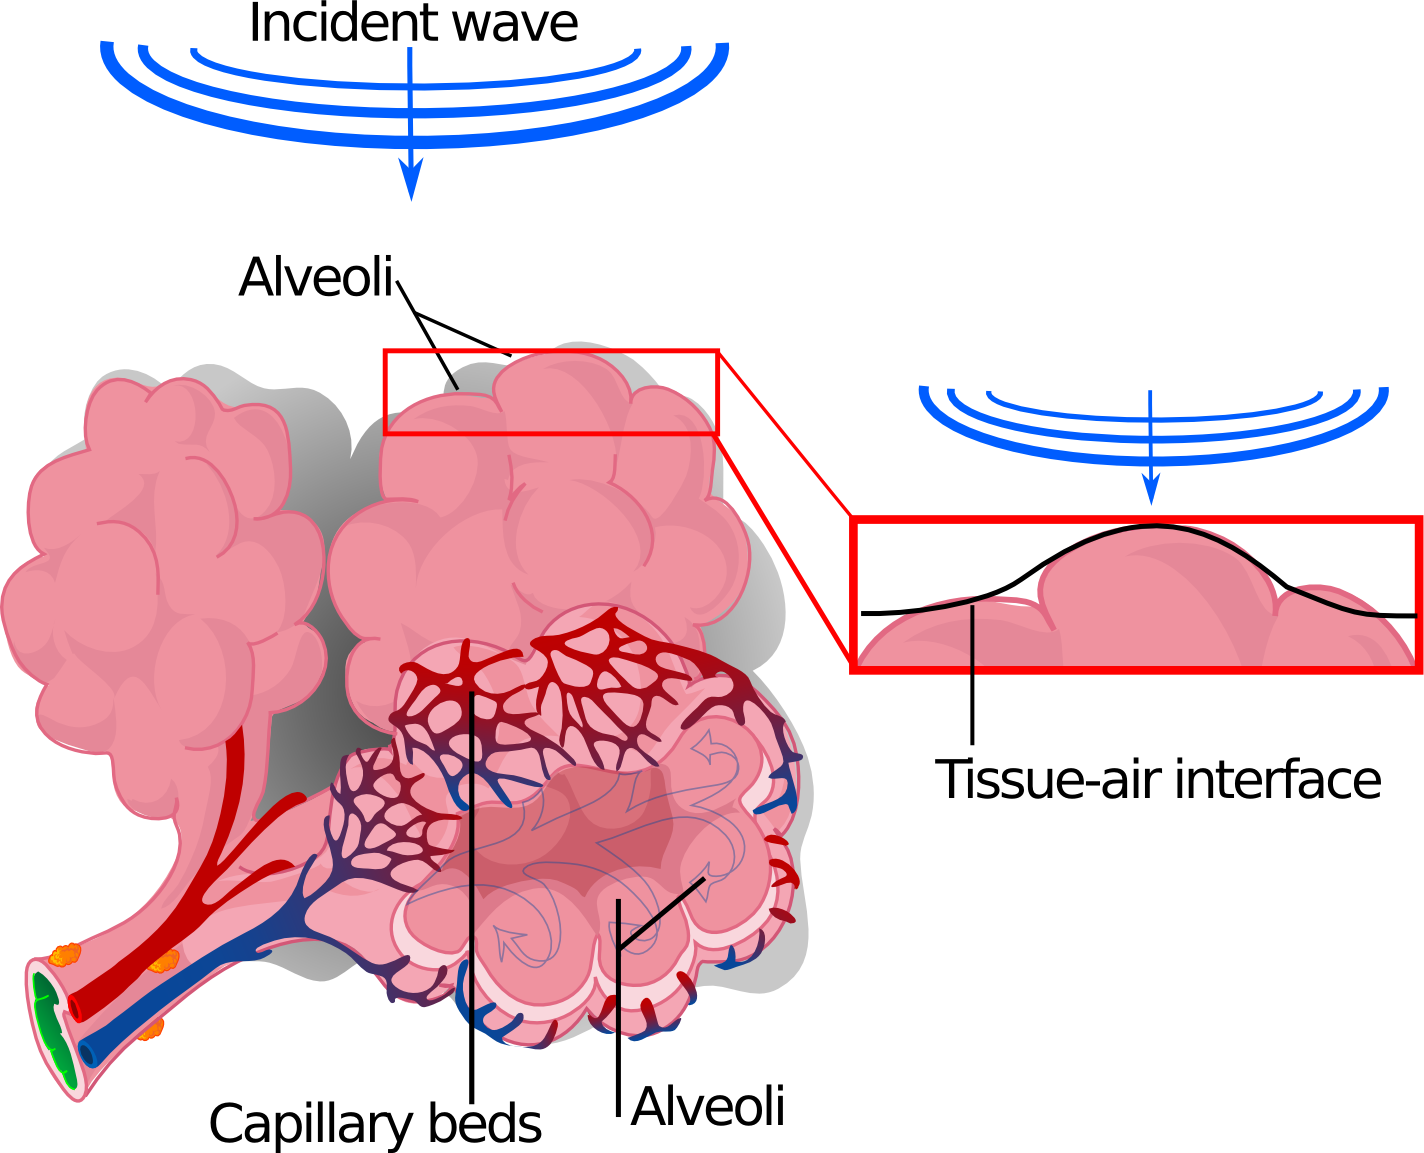
\includegraphics[width=0.48\textwidth]{./figs/lung_figs/Alveolus_US_zoom_diagram.pdf_tex} \hfill

  \def\svgwidth{0.48\textwidth}
  \import{./figs/lung_figs/}{usbe_lung_schematic2.pdf_tex} \hfill%
  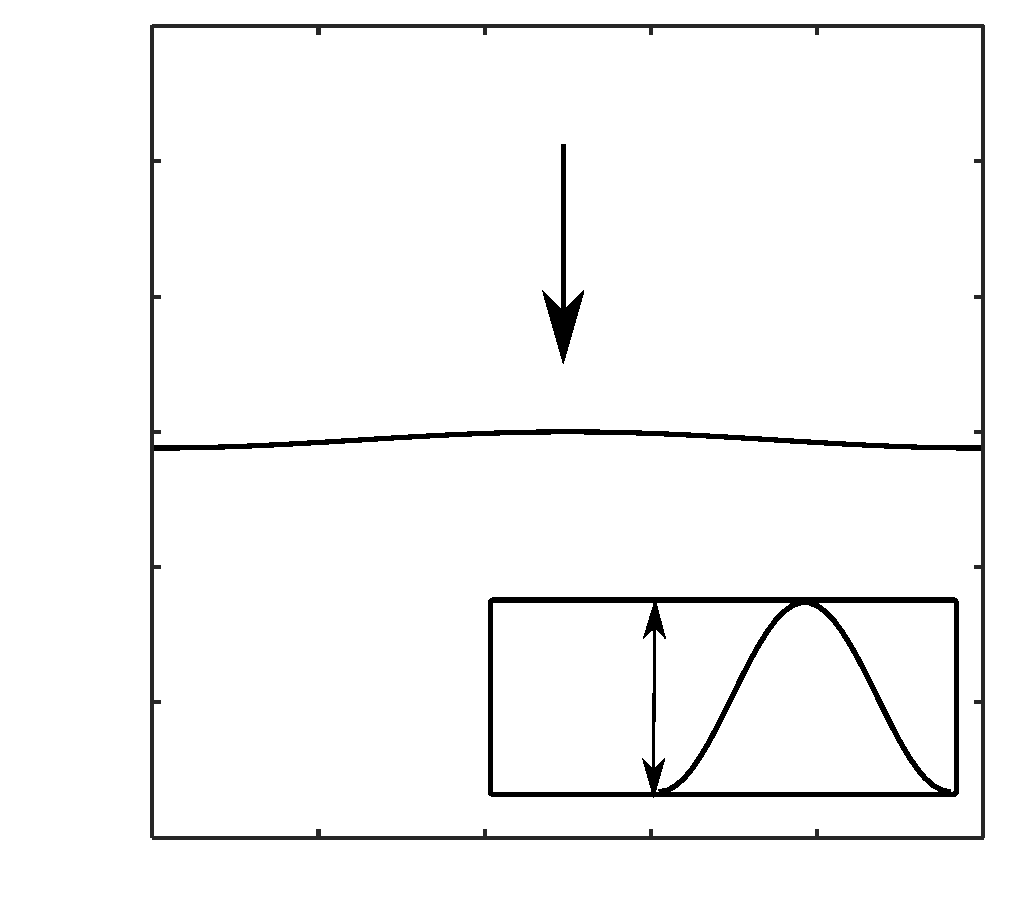
\includegraphics[width=0.48\textwidth]{./figs/lung_figs/usbe_model_schematic} \hfill
  \caption[A schematic view of lung \ac{DUS} and the model problem]{A schematic view of the physical problem (left) is shown next
    to a schematic view of initial setup and boundary conditions of the
    numerical experiments performed (right). A \ac{DUS} pulse impinging
    from tissue onto a pulmonary alveolus is modeled as an acoustic wave
    impinging from water onto a sinusoidally perturbed water-air interface.}
  \label{fig:lung_schematic}
\end{figure}
The experiments are designed to model the physics associated with a
\ac{DUS} pulse propagating from soft lung tissue (modeled as water)
onto a pulmonary alveolus (modeled as air). Accordingly, we consider a
2D, compressible inviscid fluid system in the $xy$-plane with an
acoustic wave impinging from water (top) downward toward air
(bottom). The water-air interface is initially located near $y=0$ 
and has a sinusoidal shape with wavelength $\lambda$ and amplitude
$0.03\lambda$ as seen in Figure \ref{fig:lung_schematic}. The width
of the rectangular computational domain is $1\lambda$ such that it is
traversed by a single period of the interface. This interface geometry
is consistent previous studies of the \ac{RMI}
\citep{Brouillette2002}.








To model the \ac{DUS} pulse we consider two different waveforms with
different purposes. We design the first waveform to closely resemble
a typical \ac{DUS} pulse, in order to simulate the appropriate dynamics.
The waveform shape is composed of a sinusoidal pressure modulated by a
Gaussian envelope as seen in Figure \ref{fig:p0}),
%
\begin{align} \label{eq:us_waveform}
p(t)=p_a \sin{\left( 2\pi f \left[ \left(t-t_0\right)^2\right]\right)}
\exp{\left(-\frac{t-t_0}{FWHM/\left(2\sqrt{2\ln{\left(2\right)}}\right)}\right)}.
\end{align}
%
Here $p(t)$ is the pulse pressure as a function of time, $p_a$ is the
maximum acoustic pressure, $f$ is the frequency in Hz, $t$ is time,
$t_0$ is a time offset, and $FWHM$ is the full width at half maximum
amplitude for the Gaussian envelope. The presented \ac{DUS}- pulse
waveform is given as a function of time, as is typical of \ac{US}. The
speed of sound in water is used to convert this to a spatial waveform
for the initial condition.

Because A typical \ac{DUS} pulse is mathematically complicated and not
ideal for analysis we also use a trapezoidal waveform, which is
sufficiently simple such that the relevant vorticity and interface
dynamics can be studied analytically. To design this wave, we think of
the ultrasound pulse as a sum of sin waves, each of which is composed
of half-sinusoids, which can be approximated as trapezoidal
waves. This thought process is illustrated in figure \ref{fig:p0}
(Left). Hence we use an initially symmetric trapezoidal waves.

Each wave is prescribed as an initial condition in the flow and is
composed of three stages, described here in the order that they
encounter the interface. First, compression occurs. Pressure increases
linearly from atmospheric to a maximum of $p_a=1, 5$, or $10$ MPa
gauge pressure. Second, the elevated pressure $p_a$ remains constant
over a fixed distance (or time). Third, expansion occurs and pressure
decreases linearly back to atmospheric pressure. The pressure rise and
fall occur over equal distances $5\lambda$, such that they have
constant, equal slopes $\pm p_{a}/5\lambda$. Note that this neglects
wave distortion due to acoustically induced changes in sound speed,
which we assume to be small for our purposes. Unless otherwise stated,
the period of constant pressure has length $35\lambda$. Hence the
total length $L$ of the incoming trapezoidal wave is $45\lambda$. We
assume a typical alveolar length scale $\lambda=100 \, \mu$m. For the
wave initially in water, (c=$1500$ m/s), we find an equivalent
acoustic pulse duration of our waveform is $3 \, \mu$s.  This is
within the range of typical \ac{US} pulse durations in clinical
imaging \citep{Edelman2005} and relevant research \citep{Obrien2006b}.
%
\begin{figure}% 
  \centering%
  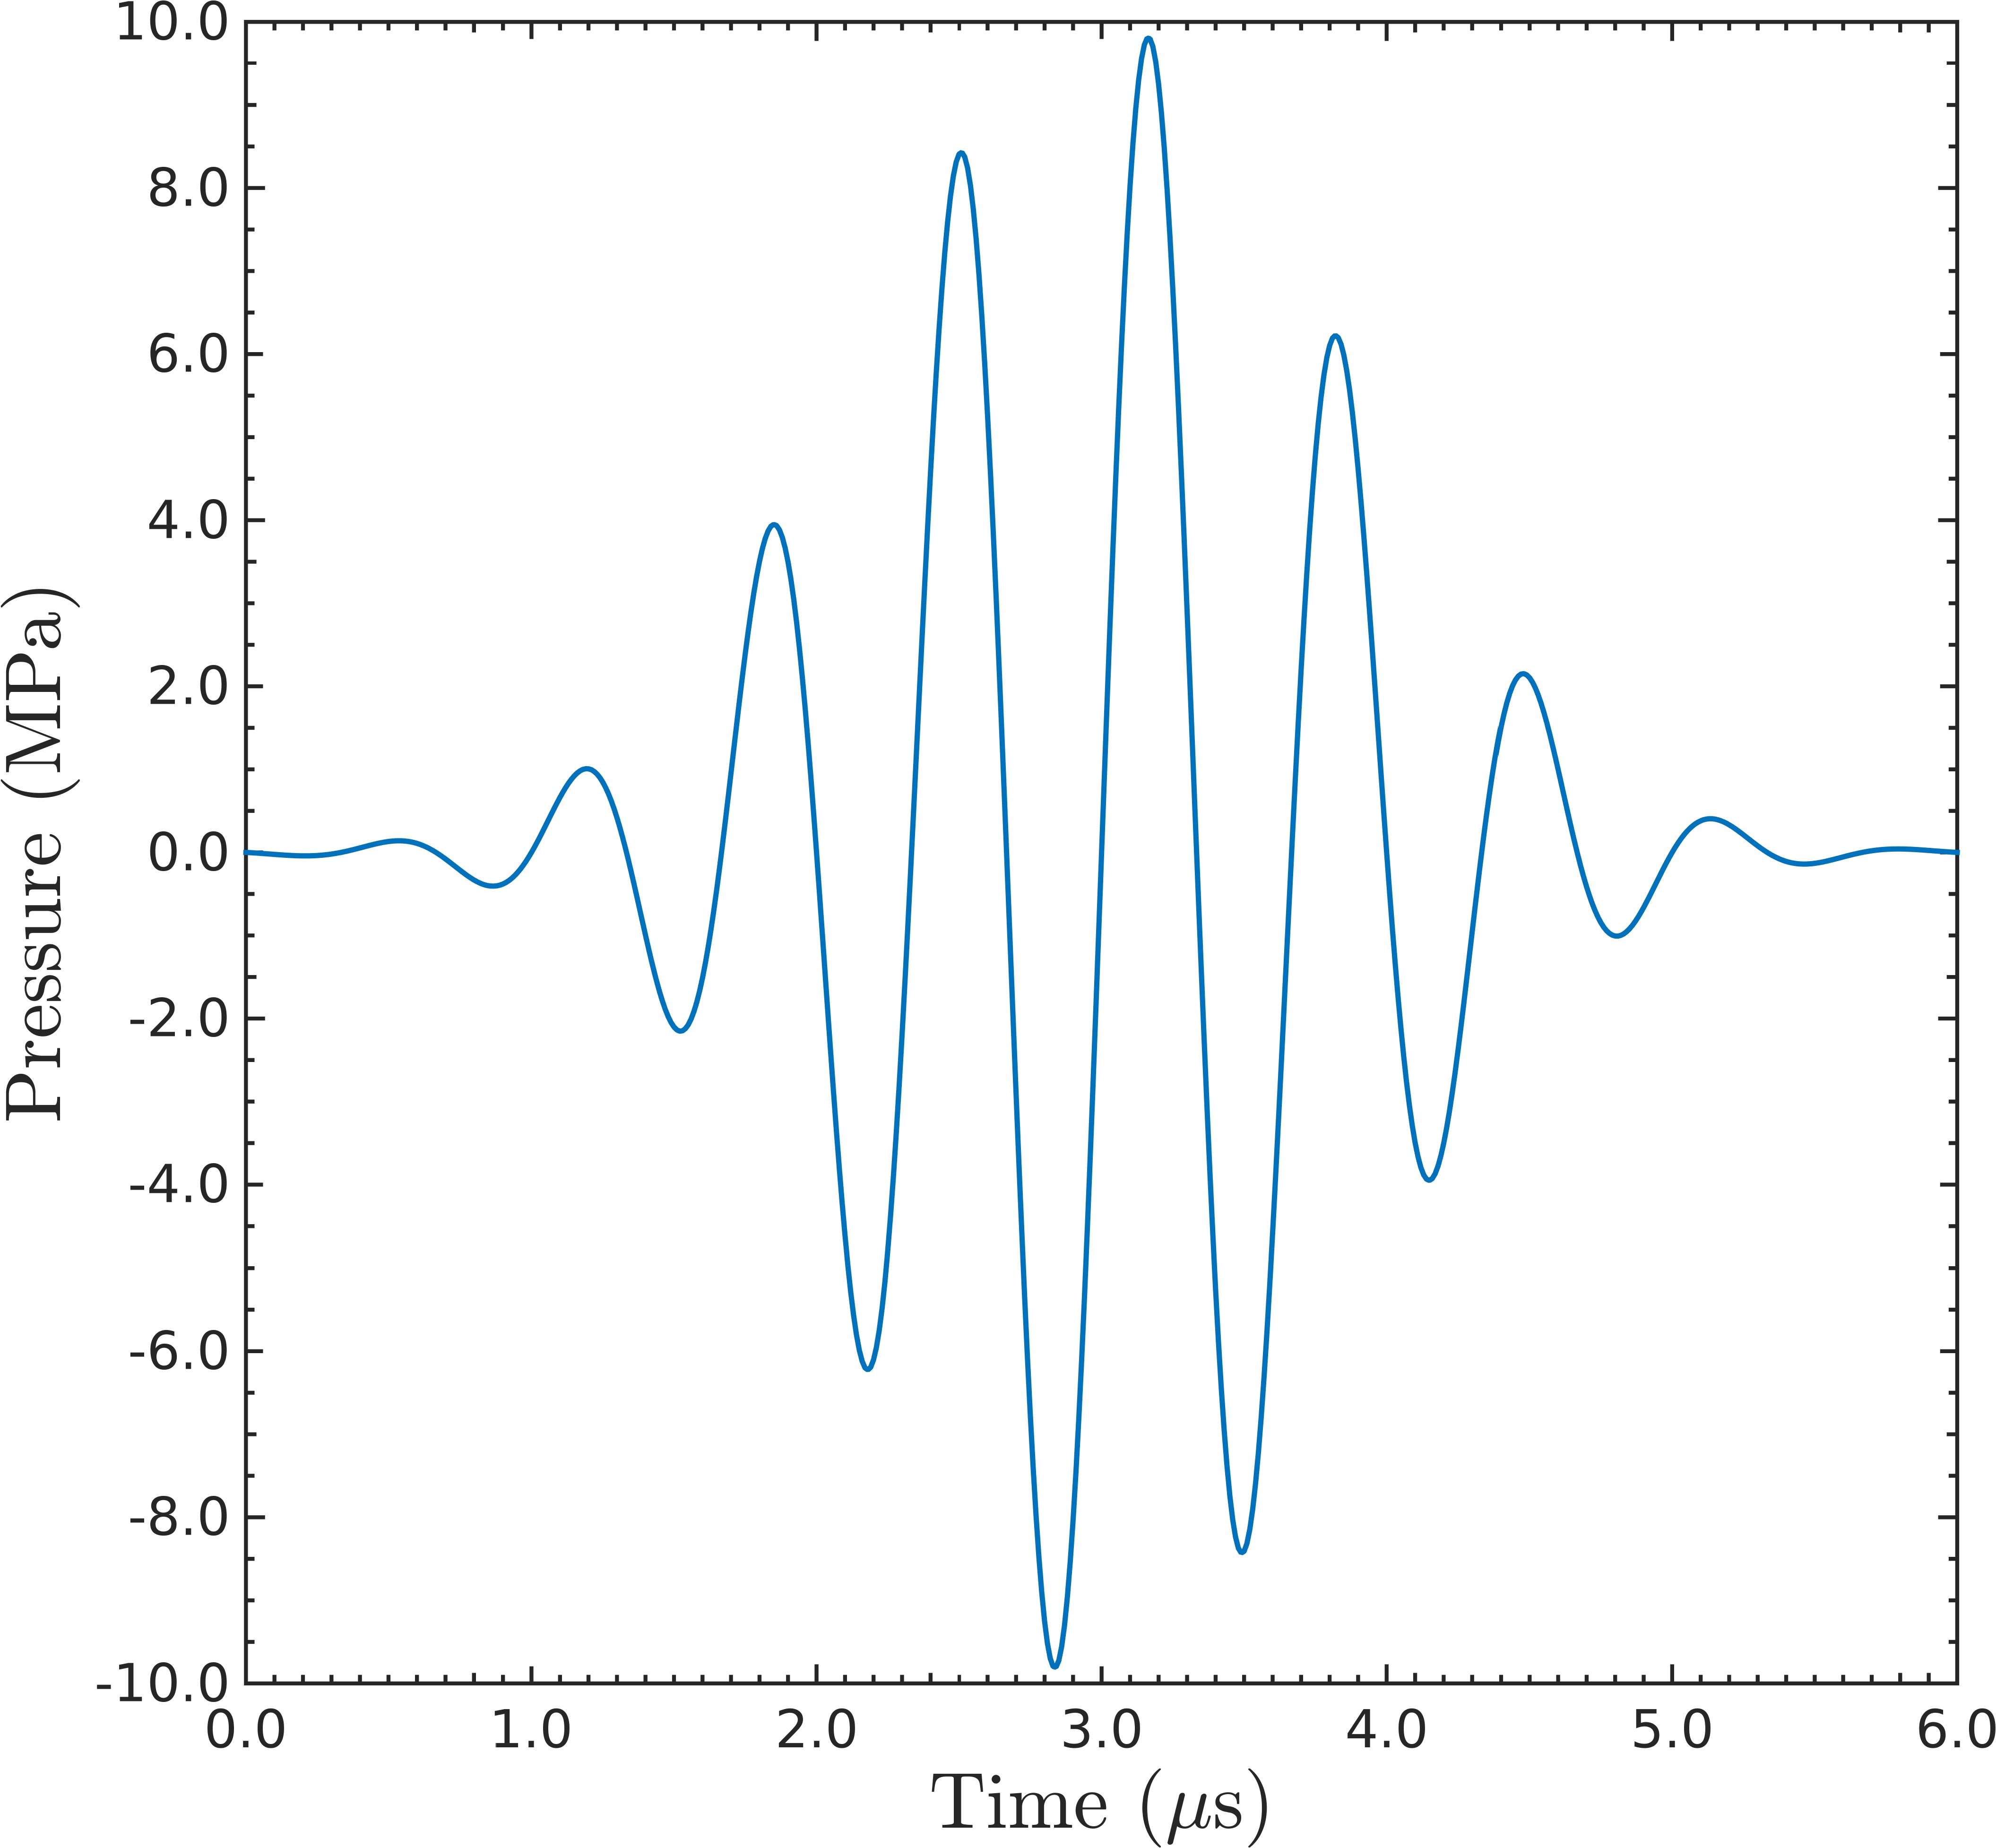
\includegraphics[width=0.32\textwidth]{./figs/lung_figs/p0_vs_t_us}\hfill%
  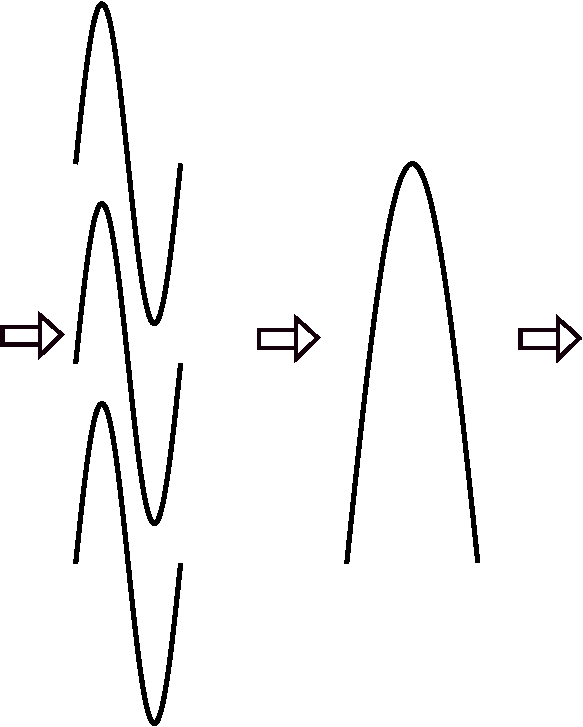
\includegraphics[width=0.17\textheight]{./figs/lung_figs/wave_logic_schematic2}\hfill
  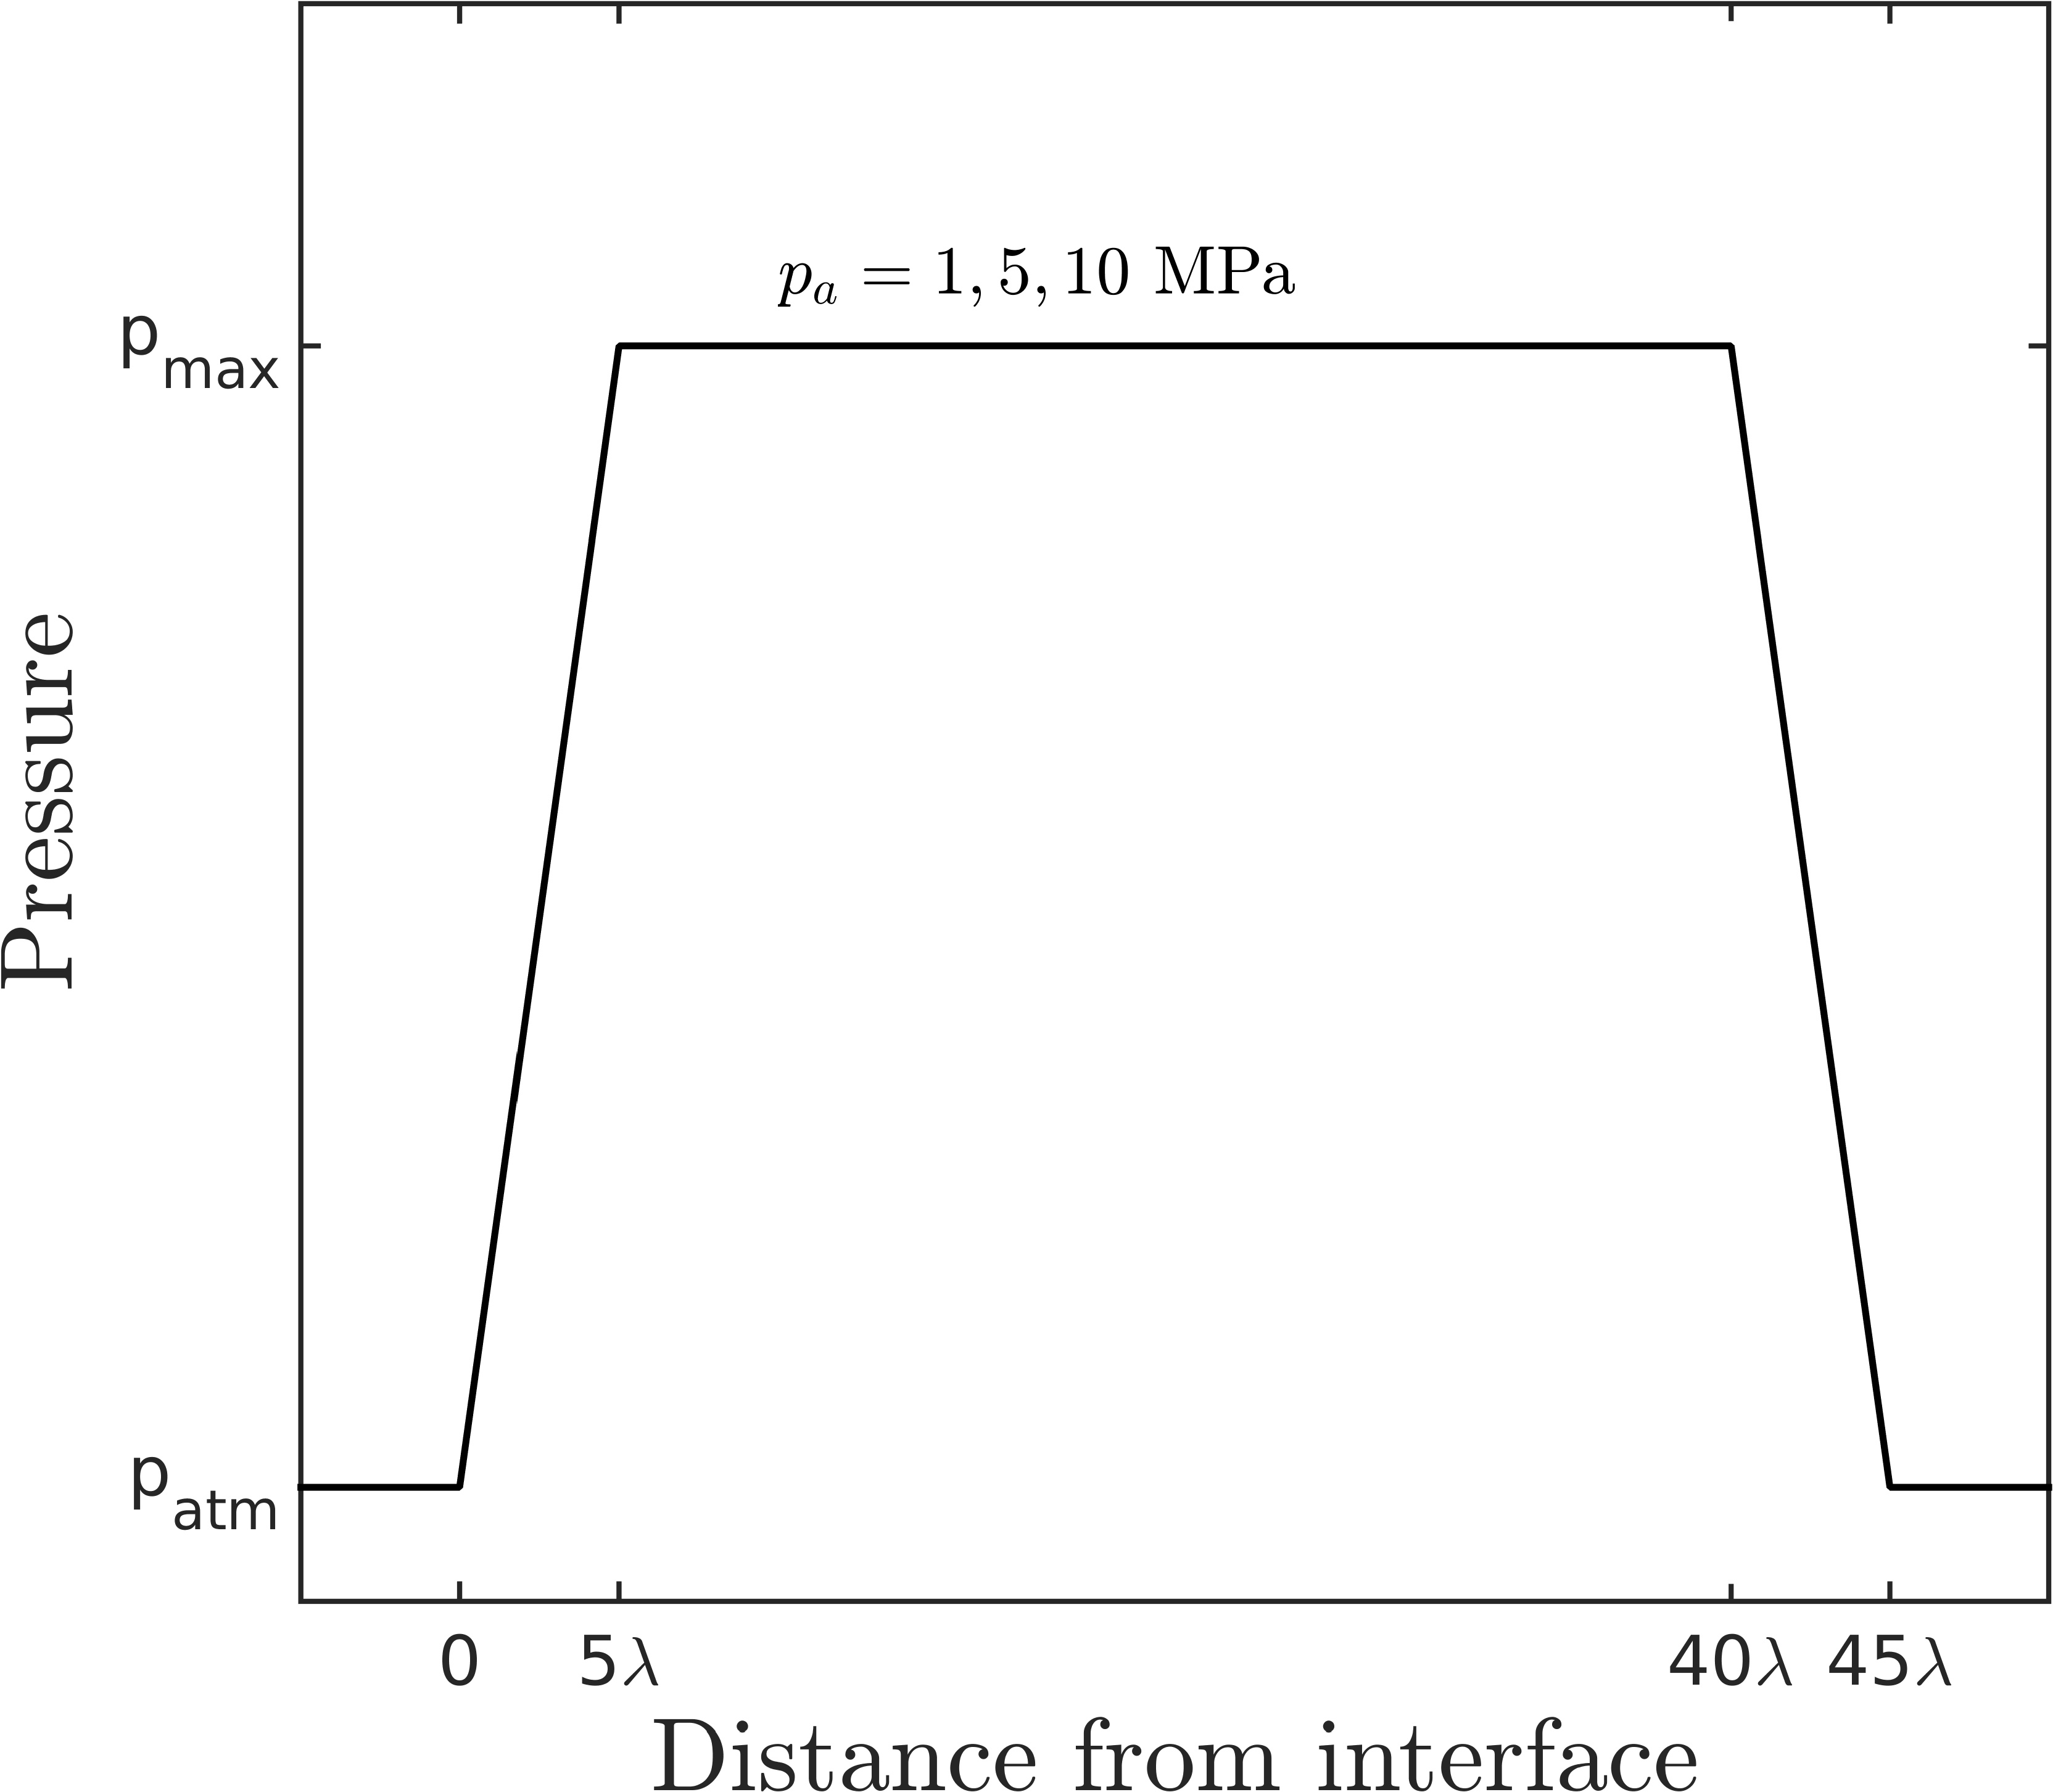
\includegraphics[width=0.32\textwidth]{./figs/lung_figs/p0_vs_y}%
  \caption[Trapezoidal and \ac{DUS} pulse waves]{The initial pressure
    waveforms in the domain. A \ac{DUS} pulse used as in initial
    condition (Left) is thought of as a sum of (half) sinusoids
    (Center), which can each be approximated as a trapezoidal waves
    (Right). The trapezoidal wave initial condition, shown as a function of
    vertical distance from the interface, is used for the bulk of this
    study.}%
  \label{fig:p0}
\end{figure}
%
\subsection{Governing equations}
The governing equations describing the dynamics \ac{US} lung
interaction are conservation of mass, momentum, and energy for a
compressible, viscoelastic material. In the present work we neglect
elastic and viscous effects to arrive at the Euler equations of fluid
motion, which we nondimensionalize by the density $\rho$ and speed of
sound $c$ of air.  For our setup we model the tissue as water and
alveolus as air and the \ac{DUS} pulse as a trapezoidal pressure
waveform. Hence we solve the Euler equations to simulate simplified
trapezoidal acoustic waves propagating from water towards a
sinusoidally perturbed water-air interface. The interface and
vorticity dynamics are studied.

It is worth noting that the Euler equations are length scale invariant, and
thus no inherent physical length scale exists in the equations that we
solve. Hence all length scales hereafter will be considered relative
to an interface perturbation wavelength $\lambda$. Within the context
of the \ac{DUS}, $\lambda$ can be thought of as a typical length scale
of an alveolus.

We solve the dimensionless Euler equations of compressible, inviscid
fluid motion in two dimensions ($x,y$),
%
\begin{subequations} \label{eq:euler}%
  \begin{align}% 
    \frac{\partial \rho}{\partial t} + \frac{\partial \left(\rho u\right)}{\partial x} + \frac{\partial \left(\rho v\right)}{\partial y} = 0,\\
    \frac{\partial \rho u}{\partial t} + \frac{\partial}{\partial x}\left( \rho u^2+p\right)  + \frac{\partial}{\partial y}\left( \rho uv\right) = 0,\\
    \frac{\partial \rho v}{\partial t} + \frac{\partial}{\partial x}\left( \rho uv\right)  + \frac{\partial}{\partial y}\left( \rho v^2+p\right) = 0,\\
    \frac{\partial E}{\partial t} + \frac{\partial}{\partial x}\left[u\left(E+p\right)\right] + \frac{\partial}{\partial y}\left[v\left(E+p\right)\right] = 0,
  \end{align}%
\end{subequations}%
%
where $t$ is time, $\rho$ is density, $p$ is the pressure, $u$ and $v$
are the velocity components in the $x$ and $y$ directions
respectively, and $E$ is the total energy. We use the density and
sound speed of air at 300 K to nondimensionalize the system. It is
worth noting that the Euler equations are length scale invariant, and
thus no inherent physical length scale exists in the equations that we
solve. Hence all length scales hereafter will be considered relative
to an interface perturbation wavelength $\lambda$.

To close the system, we solve a stiffened equation of state which
relate the total energy to the pressure and velocity in the flow, such
that,
% 
\begin{align} \label{eq:stiffened_eos}%
  E=\frac{\rho\left(u^2+v^2\right)}{2} + \frac{p+\gamma B}{\gamma-1}.
\end{align}
%
Here $B$ is a measure of liquid stiffness. For perfect gases, such as
is our treatment of air, $\gamma$ is the specific heats ratio and
$B=0$. The sound speed in our simulations is calculated based on the
following relationship, derived from the stiffened equation of state.
%
\begin{align}
  c = \sqrt{\frac{\gamma\left(p+B\right)}{\rho}}.
\end{align}
%
While physical diffusion is not considered in this setup, numerical
diffusion does occur at the water-air interface, creating a mixed
region between the two fluids. The numerical treatment of the
diffusion layer at the interface for the initial condition is such
that the density has an exponential profile \citep{Latini2007}, which
is used to get the mass fraction and molecular weight fields in the
mixed region. Which then used to determine the other material
parameters in the mixed region in a thermodynamically consistent
fashion.

To solve for
the material parameters in the mixed region and prevent spurious
pressure oscillations at the interface, two additional advection
equations are solved for $\gamma$ and $B$.
\begin{subequations} \label{usbe_lung_eosvar_advection}%
\begin{align}% 
\frac{\partial}{\partial t}\left(\frac{\gamma B}{\gamma-1}\right)+\vec{u}\frac{\partial}{\partial x}\left(\frac{\gamma B}{\gamma-1}\right) = 0,\\
\frac{\partial}{\partial t}\left(\frac{1}{\gamma-1}\right)+\vec{u}\frac{\partial}{\partial x}\left(\frac{1}{\gamma-1}\right) = 0. 
\end{align}%
\end{subequations}%
This implementation is consistent with the works of \cite{Abgrall1996,
  Shyue2001, Beig2015}. Details of this implementation are explained
by \cite{HenrydeFrahan2015}.
%
The dimensional and dimensionless values of each fluid property can be
found in tables \ref{tab:usbe_lung_dimensional_parameters} and
\ref{tab:usbe_lung_dimensionless_parameters} respectively.
% 
\begin{table}[bp]%
  \begin{center}
    \caption{Dimensional properties of air and water used in simulations.}
    \label{tab:usbe_lung_dimensional_parameters}%
    \begin{tabularx}{0.75\textwidth}{| X | X | X | X | X |}
      \hline
      & Density, $\rho^*$ (kg/m$^3$) & $\gamma$ & $B^*$ (Pa)  & $c^*$ (m/s) ($p$=$1$ atm) \\ \hline
      Air   & 1.18                        & 1.4      & 0         & 347.2     \\ \hline
      Water & 996                           & 5.5      & 492115000 & 1648.7     \\ \hline
      \multicolumn{5}{l}{\small $^*$ indicates dimensional parameter}
    \end{tabularx}
  \end{center}
\end{table}%
\begin{table}[bp]%
  \begin{center}
    \caption{Dimensionless properties of air and water used in simulations.}
    \label{tab:usbe_lung_dimensionless_parameters}%
    \begin{tabularx}{0.75\textwidth}{| X | X | X | X | X |}
      \hline
      & Density, $\rho$ & $\gamma$ & $B$ & $c$ \\ \hline
      Air   & 1                          & 1.4      & 0         & 1          \\ \hline
      Water & 846.6                      & 5.5      & 3469.1    & 4.75       \\ \hline
      \multicolumn{5}{l}{\small Parameters are nondimensionalized by the density and sound speed of air. }
    \end{tabularx}
  \end{center}
\end{table}
%
\subsection{Numerical methods}%
\label{subsec:numerical_methods}%
To solve the governing equations, we implement a third-order accurate
\ac{DG} scheme in space and a fourth-order accurate, adaptive
Runge-Kutta method to march forward in time
\citep{HenrydeFrahan2015}. Roe solver is used to calculate flux in an
out of each cell in a way that handles discontinuities and keeps the
interface sharp. As previously stated, the computational domain width
($x$-direction) is $\lambda$. The domain length ($y$-direction) is
80$\lambda$. The grid resolution is 100 points per $\lambda$ unless
otherwise stated. To minimize artificial reflections, we use inflow
and outflow boundary conditions at the top and bottom of the domain,
and implement geometric grid stretching in the vertical direction for
the top and bottom-most 10$\lambda$ segments of the grid. Periodic
boundary conditions are used at the left and right edges of the
domain.

%%% Local Variables:
%%% mode: latex
%%% TeX-master: "../../prelim"
%%% End:
